\documentclass[a4paper,11pt]{article}

\usepackage[utf8]{inputenc}

\usepackage{graphicx}
\usepackage{caption}
\usepackage{subcaption}

\usepackage{hyperref}

\usepackage{pgfplots}
\pgfplotsset{compat=1.18} 

\usepackage{minted}

\begin{document}

\title{
    \textbf{Assignment 6 Report - Queue in Java}
}
\author{Dean Tsankov}
\date{\today}

\maketitle

\section*{Introduction}

In this report we will take a look at a very common data structure that behaves quite similarly to an every day life occurrence in our lives. This said structure is a queue - a row of items forming a line. This is, it is ordered so that when an item is added to the queue it will have to wait for all other items in the queue to be removed before it can be accessed. Queues are also referred ta as a FIFO structure, first-in-first-out, which simply describes the functionality. This can be compared to a stack which is in turn referred to as LIFO (last-in-first-out) structure. 
\\

We will achieve a queue implementation by using a linked list. This underlying structure would be quite easy to implement and work with. It should also be quite efficient although by design it will allocate and de-allocate data structures in each operation.

\section*{The linked list implemented queue}

For a queue only one property is needed, a head, pointing to the first element in its list of items. When an element is enqueued it goes to the end of this list and later items are dequeued from the beginning. My queue goes on to implement the following methods in addition to the provided beginning of the structure:

\begin{minted}[
frame=single,
framesep=2mm,
baselinestretch=1.2,
fontsize=\footnotesize,
]{java}
    (...)
    public void enqueue(T item) {
        Node n = new Node(item, null);

        Node nxt = this.head;
        if (nxt == null) {
            this.head = n;
        }else{
            while (nxt.next != null) {
                nxt = nxt.next;
            }
            nxt.next = n;
        }
    }
    (...)
\end{minted}

As stated to enqueue an element we have to go trough all entries in the queue to find the last previously added one in order to give it a reference to the new. There is also a check whether the queue is empty when adding in order to prevent a null pointer exception. Implemented this way, we can notice that with the growth of the queue so too will the execution time grow, since we always do a traversal. Meaning we could expect an {\tt O(n)} complexity.  

\begin{minted}[
frame=single,
framesep=2mm,
baselinestretch=1.2,
fontsize=\footnotesize,
]{java}
    (...)
    public T dequeue() {
        if(this.head!=null){
            Node temp = this.head;
            this.head = this.head.next;
            temp.next = null;
            return temp.item;
        } else {
            return null;
        }
    }
    (...)
\end{minted}

Dequeue-ing in this implementation turns out to be quite simple in terms of operations. We make the node the current head is pointing to (as its {\tt next} property) the new head, and return the value of the previous head. There is also a check if there are no longer any elements to dequeue. All these operations happen in constant time and as such this method should have {\tt O(1)} time complexity.

\subsection*{Benchmark}

The following graph fulfils the predictions for the behaviour of the enqueue function for this queue implementation.

\begin{figure}[H]
    \centering
    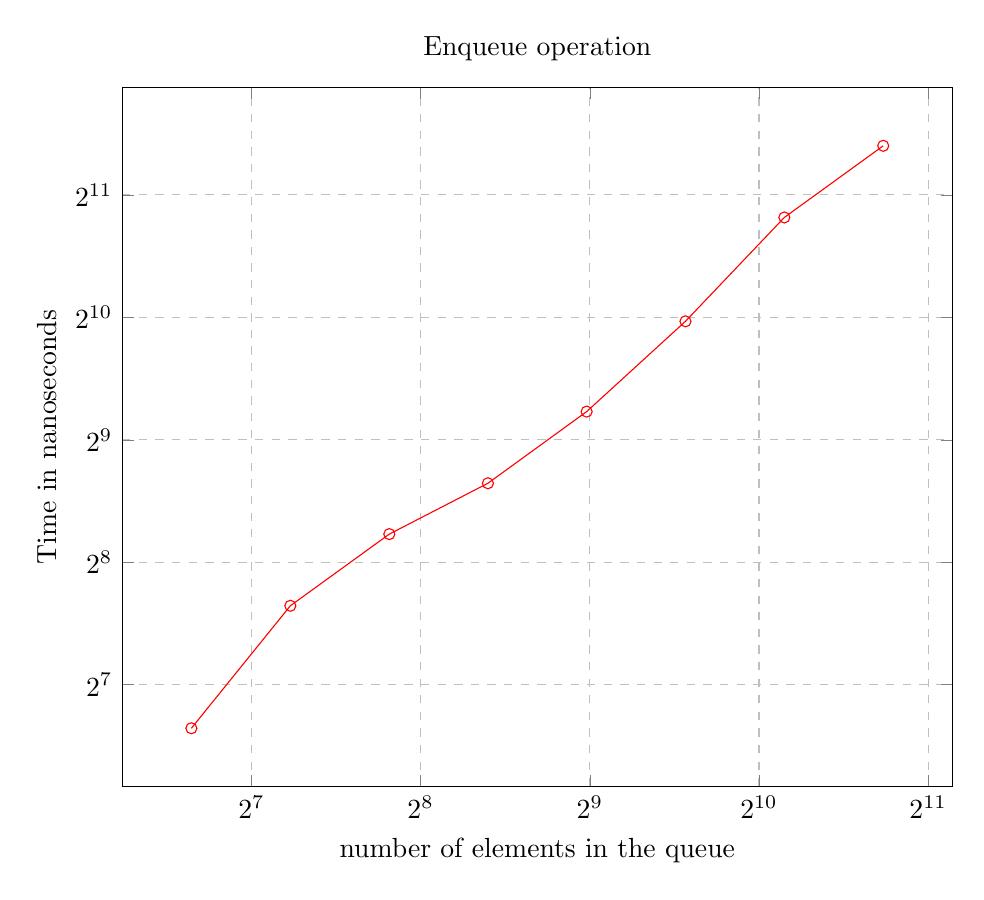
\begin{tikzpicture}
        \begin{axis}[
            title={Enqueue operation},
            width=\linewidth,
            xlabel={number of elements in the queue},
            ylabel={Time in nanoseconds},
            xmode=log,
            log basis x={2},
            ymode=log,
            log basis y={2},
            ymajorgrids=true,
            xmajorgrids=true,
            grid style=dashed,
        ]
        
        \addplot[
            color=red,
            mark=o,
            ]
            coordinates {
            (100,100)(150,200)(225,300)(337,400)(505,600)(757,1000)(1135,1800)(1702,2700)
            };
            
            
        \end{axis}
        \end{tikzpicture}
    \caption{Enqueue operation benchmark}
    \label{fig:plot1}
\end{figure}

\section*{Improvement}

It might not be hard to spot that if instead of having the head pointer keep track of the first added element and go down the queue each time we want to add an element, we could have the head point to the last added element. This way when enqueue-ing we simply have to give the head's next reference to be the new addition and make it itself the head. This now makes the enqueue operation work for constant time, but conversely the dequeue's complexity grows linearly. 
\\

Following this in order to improve the algorithm, our Queue structure could just keep a pointer for both the first and last added elements and with the respective operations change them accordingly. The two said functions would look as follows:

\begin{minted}[
frame=single,
framesep=2mm,
baselinestretch=1.2,
fontsize=\footnotesize,
]{java}
    (...)
    public void enqueue(T item) {
        Node n = new Node(item, null);

        if (this.tail != null) {
            this.tail.next = n;
        } else {
            this.head = n;
        }
        this.tail = n;
    }
    (...)
\end{minted}

Here we add an element by either giving it as the current tail's next reference and making it the new tail or making it both the head and the tail depending on whether this is the first added element to the queue or not. 

\begin{minted}[
frame=single,
framesep=2mm,
baselinestretch=1.2,
fontsize=\footnotesize,
]{java}
    (...)
    public T dequeue() {
        ...
    (...)
\end{minted}

Removing an element has the exact same form as the above implementation and so as such is not pasted here again.

\subsection*{Benchmark}

Now with this improvement we should expect the all around linear time complexity. The graph below confirms these thought.  

\begin{figure}[H]
    \centering
    \begin{tikzpicture}
        \begin{axis}[
            title={Improved Enqueue operation},
            width=\linewidth,
            xlabel={number of elements in the queue},
            ylabel={Time in nanoseconds},
            xmode=log,
            log basis x={2},
            ymode=log,
            log basis y={2},
            ymajorgrids=true,
            xmajorgrids=true,
            grid style=dashed,
        ]
        
        \addplot[
            color=blue,
            mark=o,
            ]
            coordinates {
            (100,1)(150,1)(225,1)(337,1)(505,1)(757,1)(1135,1)(1702,1)
            };
            
            
        \end{axis}
        \end{tikzpicture}
    \caption{Improved Enqueue operation benchmark}
    \label{fig:plot1}
\end{figure}

\section{Conclusion}
Understanding how a queue works allows us to add it to the arsenal of data structures we are acquiring. Each of which has its own circumstances and specific behavior which can benefit a particular use case.


\end{document}